%update: Jan 15 fixed figure/table numbers, fixed figure captions.  
%update: Jan 14 fixed grammar according to prof notes
%update: Jan 13 prof rewrite for ithenticate
%update: Jan 11 table 3.1 fixed
%update: Jan 09-11 prof check
%update: Jan 03 table ok. 
%update: Nov 21 fixed equation part. 
%update: Nov 09 by professor, rewrote all text. 

%\begin{savequote}[75mm] 
%It's rather easy to play any musical instrument: all you have to do is to touch the right key at the right time and the instrument will play itself.
%\qauthor{Johann Sebastian Bach} 
%\end{savequote}

\chapter{Nanoarchitechtonics of Axial Nanowire Junctions of CdS and p-Si}

\newthought{A delicate, high-precision technique} was implemented to build and analyze axial nanowire heterojunctions inside a high-resolution transmission electron microscope (HRTEM). Through {\em in-tandem} using of a sharp tungsten probe as the nanomanipulator and an optical fiber as the optical waveguide the nanoscale CdS/p-Si axial nanowire junctions were constructed, and \textit{in situ} recorded photocurrents from them were detected. Compared to the individual constituting nanowires, the CdS/p-Si axial nanowire junctions exhibit a photocurrent saturation effect which protects them from damage under high voltages. In addition, a set of experiments demonstrates the certain relationship between the saturation photocurrent values and the incident light intensities. The designed technique is envisaged to be valuable for bottom-up nanodevice fabrications, and the documented photocurrent saturation feature should solve the Joule heating-induced failure problem in nanowire-based optoelectronic devices caused by a fluctuating bias. 

\begin{figure}  
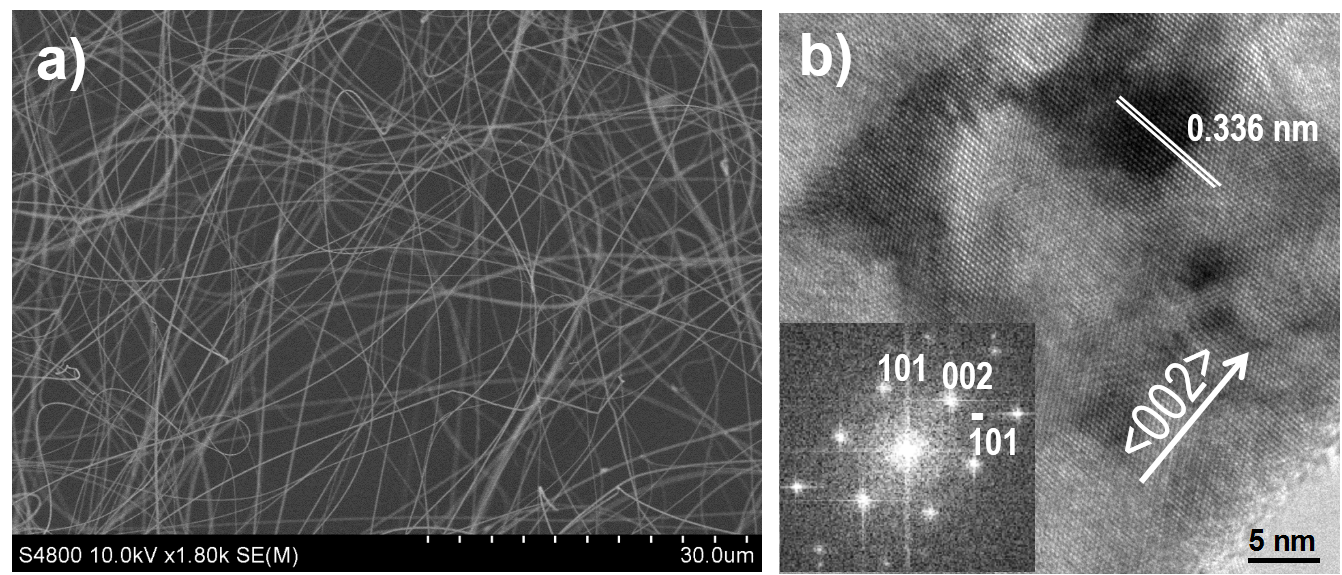
\includegraphics[width=\textwidth]{figures/figure3_s1}
\caption[SEM and TEM of CdS nanowires.]{(a) SEM image of CdS nanowires. (b) TEM image and corresponding fast Fourier
transform pattern of an individual CdS nanowire. 
\label{fig:fig3_s1}}
\end{figure}

\section{Introduction}
These days, the the key progresses in nanoscale photonics and electronics are made thanks to the significant improvement of device functions and performances. Nanowires, as prime building blocks in the bottom-up technology, have been shown to be the key candidates for the next generation booming nanophotonic applications because of their good crystallinity, high carrier mobility, confinement effects and infinite possibilities of assembling any required architecture for diverse utilizations \cite{lieberprogramable2014,tsai2014,zhangx2014}. However, till now, fabrication of a desired nanoarchitecture employing nanoscale building blocks has been a challenge. Several nanowire-based devices, such as transistors \cite{577926446,577926447,577926448}, diodes \cite{577926449}, photodetectors \cite{577926451,577926452} and logic circuits \cite{577926453,577926454}, have successfully been constructed on substrates through diverse lithography techniques. By contrast, controlled manipulation with two or more individual objects with a nanoscale precision and on-site creation of axial heteroarchitectures made of them (for the immediate optoelectronic probing) has never been tried. Building of the regarded junctions and \textit{in situ} testing of their optoelectronic characteristics must be highly important in relation to the “nanoarhitectonics” concept and uncovering novel physical properties and phenomena.\\ 

Cadmium sulfide (CdS) is known as one of the key materials in heterostructured type solar cells because of its advantageous type II window band structure  \cite{577926455}. Also, it was shown that merging CdS and Si materials must create a decent junction. Therefore, numerous new functions and  utilizations may be envisioned. In addition, a careful study revealed that CdS/p-type-Si junctions are basically better than CdS/n-type-Si junctions for rectifying properties because of their specific type II band structure \cite{577926457}. Nevertheless, reliable usage of these two "hot" optical materials, i.e. CdS and Si, is rather rare, because both junction constituents are not transparent to a solar light. And the normal layered structures are considered not to be efficient. In order to directly expose the heterojunctions to the light, a smart way is to build the nanowire array structures \cite{577926458,577926459}. In addition to the wide-spread core-shell nanowire ensembles, constructing axial nanowire heterojunctions by means of two semiconducting materials is a promising experimental route.\\

\begin{figure}
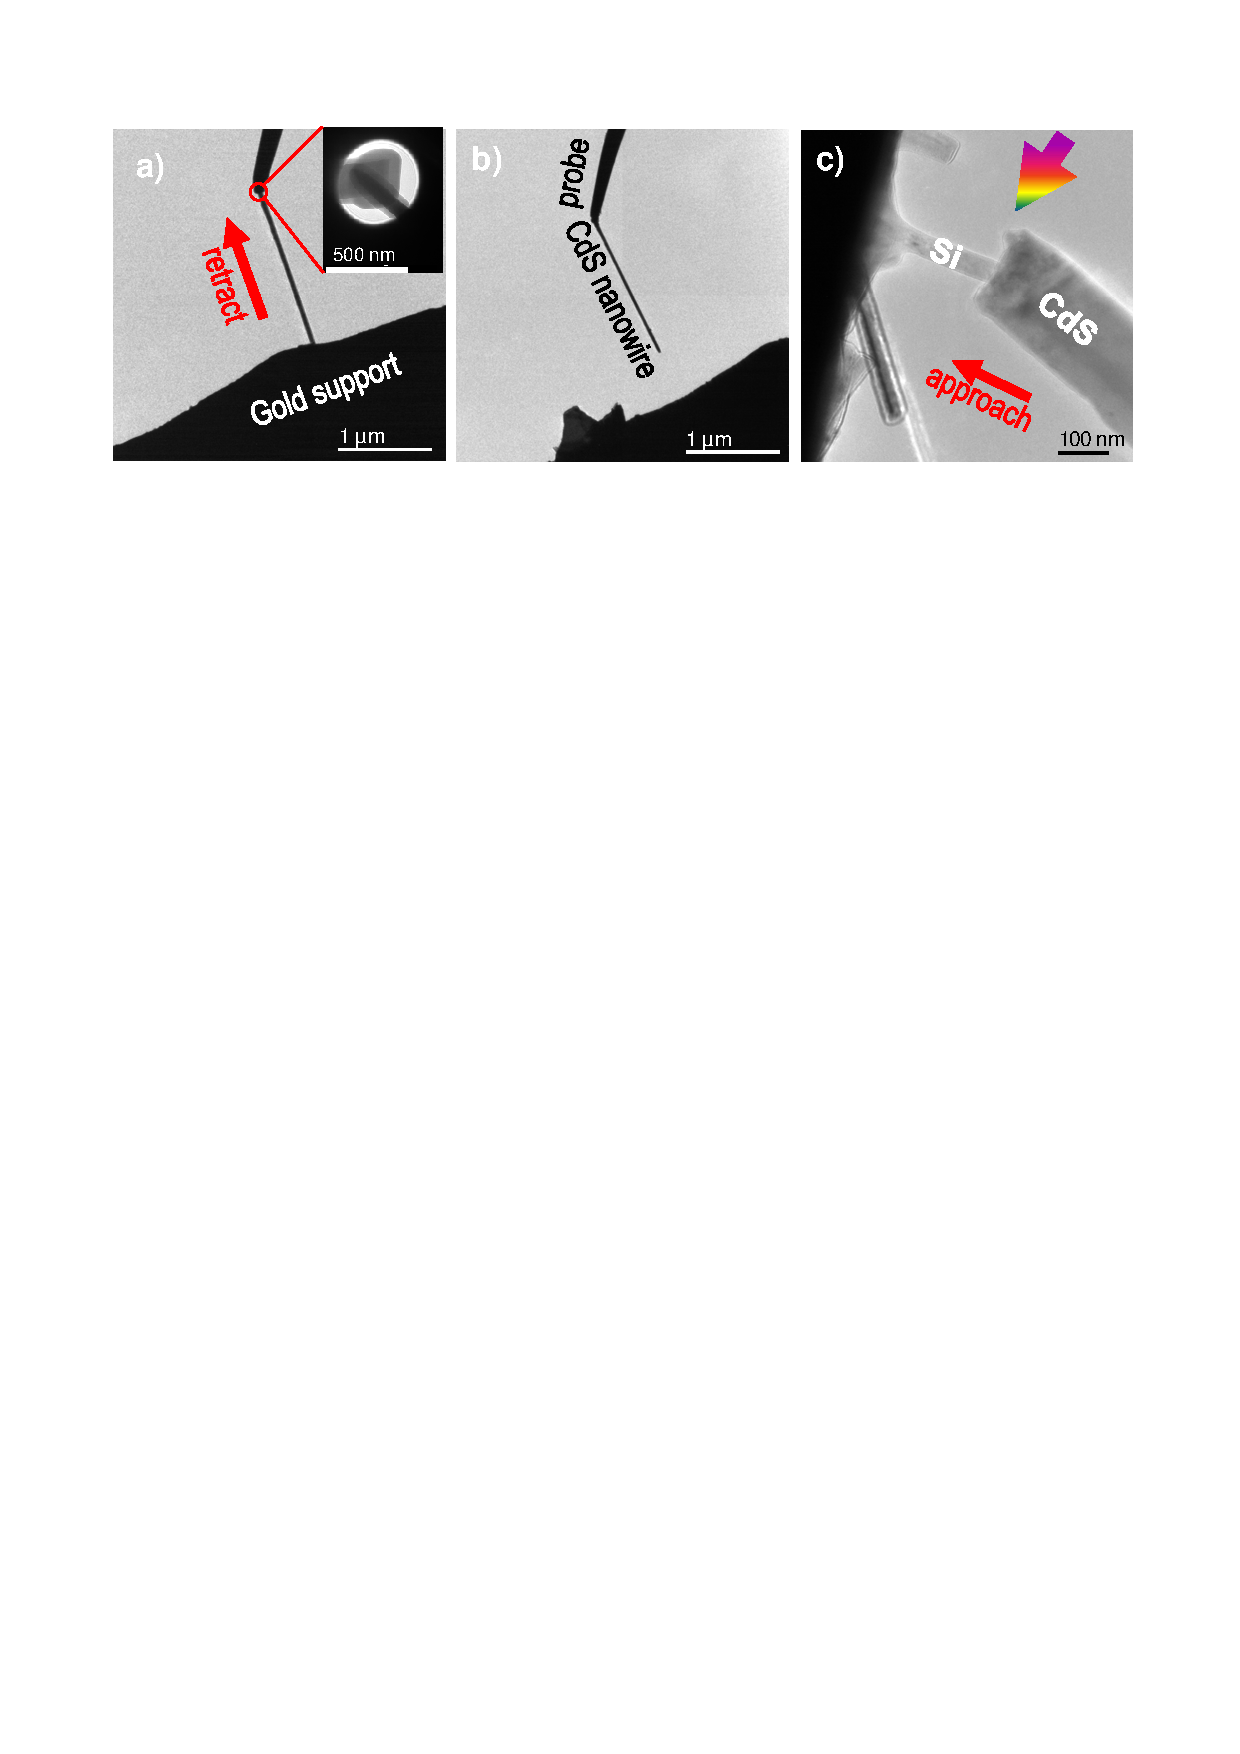
\includegraphics[width=\textwidth]{figures/figure3_1}
\caption[Making an axial junction.]{\textit{In situ} TEM images illustrating the construction of an axial CdS/p-Si nanowire junction during manipulations in HRTEM. (a) Achieving a physical contact of a piezo-driven sharp W probe with an individual clean CdS nanowire on an Au support during the first stage of the process; the inset depicts soldering the W probe and the wire under convergent electron beam irradiation. (b) Retracting the nanowire from the Au support; (c) Attaching a CdS nanowire to the individual boron-doped Si nanowire during the second stage of the manipulation. The incoming light illuminating the junction is shown with an arrow.
\label{fig:fig3_1}}
\end{figure}

Following previously made axial nanowire heterojunctions for diverse optoelectronic applications, CdS nanowires and B-doped Si nanowires have been selected by me as the targeting building blocks. Thus, in this Chapter, I demonstrate an accurate nanomanipulation technique pioneered in a HRTEM for building new axial nanowire architectures. Direct \emph{in situ} electronic and optoelectronic tests are then performed on them using the light of various wavelengths illuminating the objects of interest in TEM. The careful experiments allow me to also simultaneously have an entire control over the crystallography and spatially-resolved chemistry of the two constituting domains and their interfacial region before, during and after optoelectronic probing with high spatial and temporal resolutions specifically peculiar to HRTEM. 
My experiments reveal clear photosensing properties of the axial CdS/p-Si nanowire junctions. The latter demonstrate selective sensitivity to blue and purple lights rather than to the light of larger wavelengths. Also, the junctions display a photocurrent saturation effect. This implies that such junctions are applicable for detection of light intensities due to their low energy consumption and stability under unexpectedly pulsing biases. 
\vfill % otherwise it looks bad between figure and text here - zc. 

\section{Experimental}
\subsection{Material Synthesis}
The CdS nanowires were prepared using an Au-catalysed vapor-liquid-solid (VLS) synthesis  in a chemical vapor deposition (CVD) system, which is analogous to that used in many works \cite{zhang2014photosensing,577926461}. 1 gram of a CdS powder (99.995\%) was put on a graphite plate in the tubular furnace center as the source material. A (100) Si wafer covered with a 10 nm thick Au film was put on the other graphite piece located downstream, at a distance of 11.5 cm from the tube center. The tube was purged under N2 flow at 200 °C for 2 h, and then heated to 1000 °C at a rate of 30 °C per min. After 30 min of synthesis, the furnace was naturally cooled down to room temperature. The process proceeded under a \ce{N2} flow of 300 sccm. A wool-like yellowish product was found on the Si substrate after cooling. 
Si nanowires were fabricated via VLS mechanism in a separate CVD system. Au particles of 3 nm in diameter were taken as a metal catalyst. The boron-doped nanowires were directly prepared onto Au-coated (111) Si substrates at 600°C for 30 min in a flowing 19 sccm of \ce{SiH4} as a Si reactant gas, and diborane (\ce{B2H6}) was employed as a B precursor. The \ce{B2H6} flow in \ce{H2} was 0.2 sccm and 30 sccm of \ce{N2} served as the carrier gas. Other details related to boron-doped Si nanowires characterizations were presented in the literature. \cite{577926462,577926464,577926465}.

\begin{figure} 
\centering
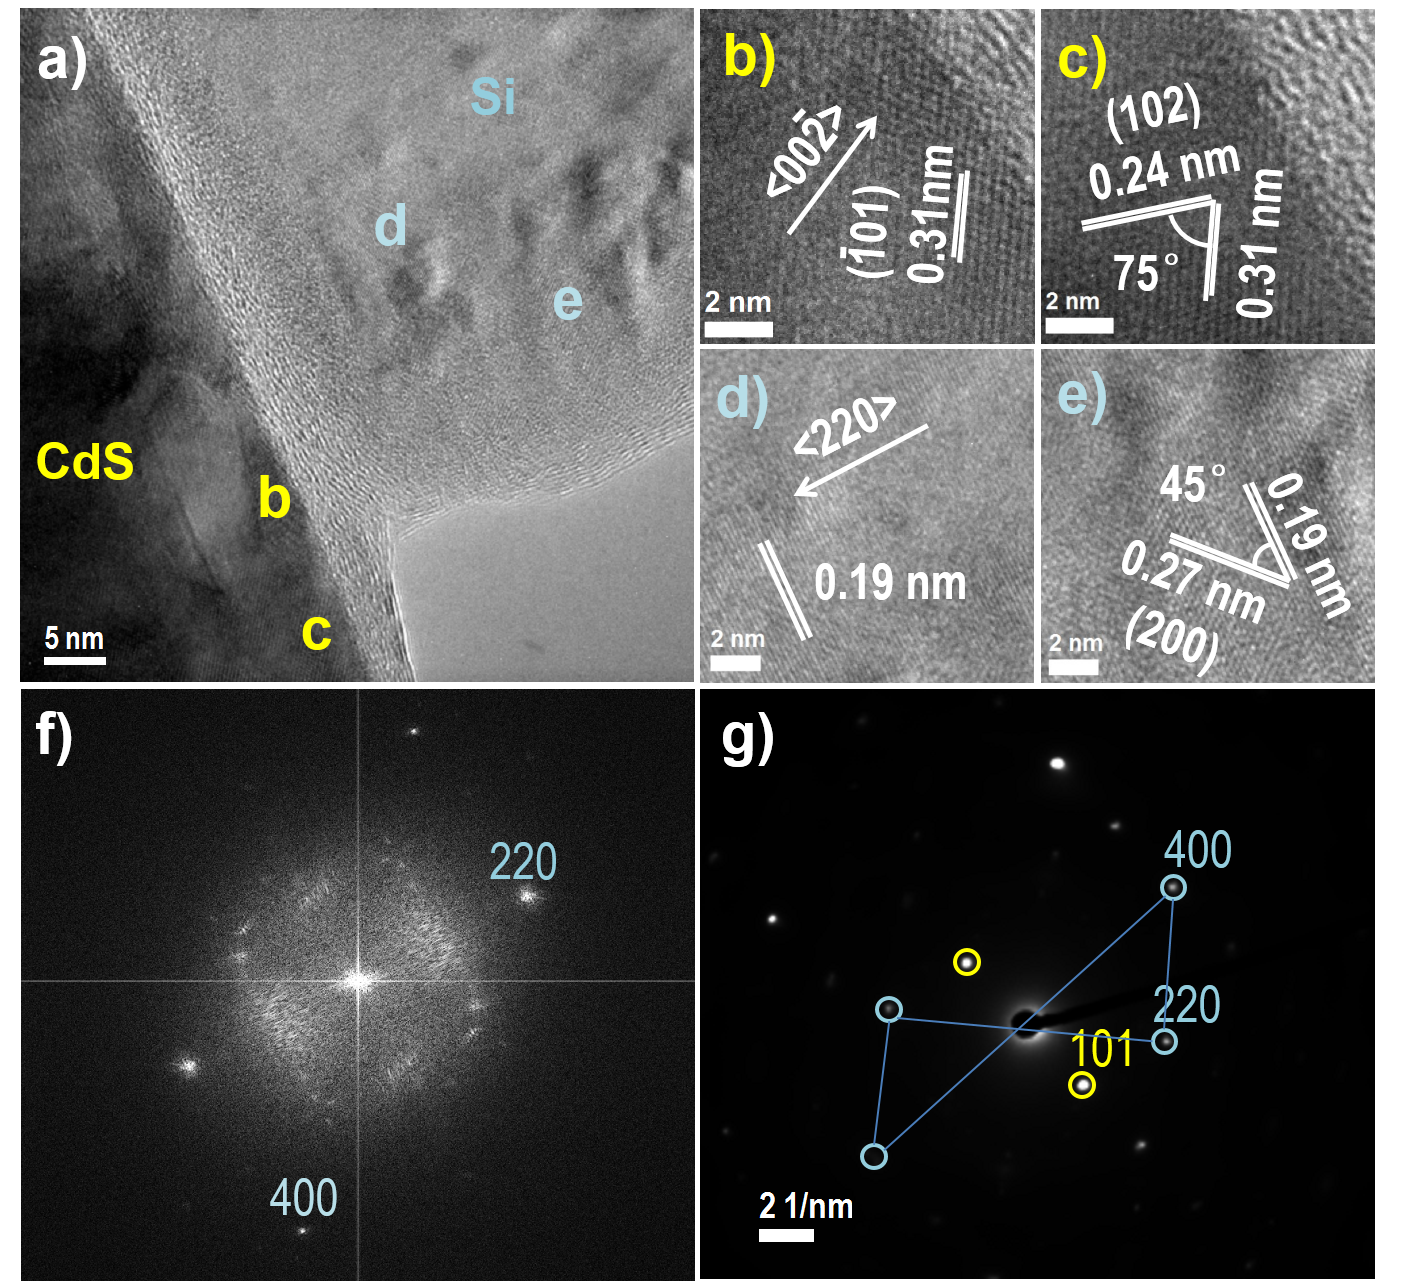
\includegraphics[width=0.6\textwidth]{figures/figure3_2}
\caption[HRTEM analysis on junction.]{(a) Overall HRTEM image of the interfacial portion of the produced CdS-p-Si junction; (b)–(e) HRTEM images acquired in the areas marked in (a); these reveal the single-crystalline nature of both nanowire segments, and (f), (g) corresponding FFT pattern and selected area electron diffraction pattern (SAED) taken from the interface. Peculiar crystallographic orientations (b)–(e) and diffraction spots (f), (g) are marked.
\label{fig:fig3_2}}
\end{figure}

\subsection{Techniques}
Field-emission scanning electron microscopy (FE-SEM) of the prepared nanostructures was performed on a Hitachi S-4800 FE-SEM operated at 10 kV. HRTEM analysis and {\em in situ} experiments were carried out using an optimized piezo-driven optical TEM holder, which is discribed in detail in Chapter 2, in an energy-filtering 300 kV JEM 3100FEF (Omega Filter) high-resolution TEM. The multimode fiber (Nanonics Imaging, Ltd.) was threaded through the holder inner channel. The fiber was connected to four laser diodes, with 405, 488, 638 and 808 nm wavelengths, and a tunable power and temperature (Thorlabs, Inc.) were used. \\

The working temperatures of laser diodes were set at 30°C. Firstly, the numerous CdS nanowires were placed onto a fresh-cut flattened Au tip covered with an electrically conductive Ag epoxy under the flash tip immersing into the CdS nanopowder sample. After heating the paint, the Au tip with the specimen was placed within the sample holder. The ultrasharp W probes used as counter-electrodes and manipulators were prepared under NaOH electrochemical etching. The W tip movements were controlled inside TEM in 3 dimensions using a piezoelectric motor for making a contact, and to test and retract the selected CdS nanowires which had been conveniently oriented with respect to the manipulator. Then the construction of axial CdS/p-Si nanowire junctions was gently performed in two steps, as described below. Typically, prior to contacting the two nanowire building blocks, an electron beam was applied to focus on the tip-ends of both CdS and p-Si nanowires for 30 s to clean the surfaces. The current–voltage (I–V) curves were recorded by using a Keithley 2612B sourcemeter. The electron beam was deliberately blanked during obtaining the quantitative current data. 

\section{Results and discussions}
As depicted in SEM image of Figure \ref{fig:fig3_s1}a, prepared CdS nanowires, $>50$ μm long, were evenly distributed over a Si substrate over a large area. In Figure \ref{fig:fig3_s1}b, a high-resolution TEM image and the fast Fourier transform pattern (FFT) confirm that an individual nanowire has a well-crystallized hexagonal structure. The growth direction is parallel to the $c$-axis and the lattice parameter $c = 0.672$ nm. 

\begin{figure}  
\centering
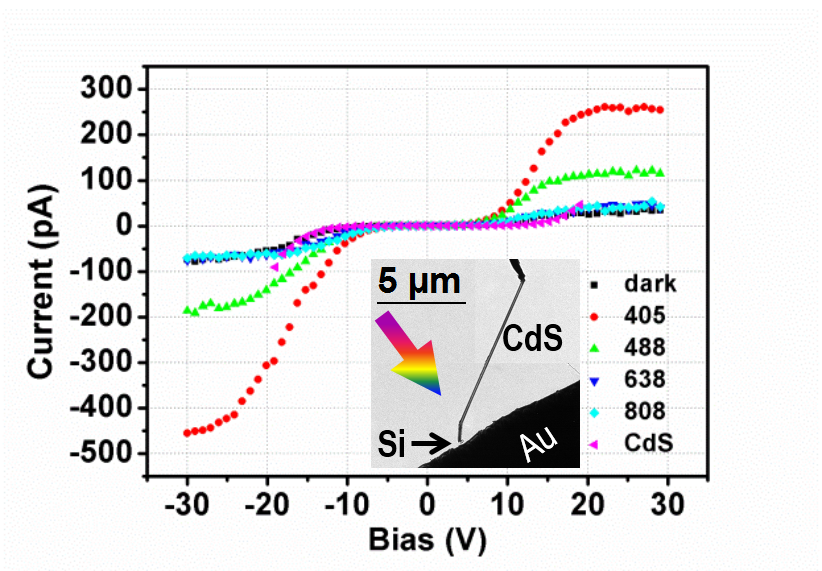
\includegraphics[width=0.6\textwidth]{figures/figure3_3}
\caption[Photocurrent through junction.]{A photocurrent outcome of an individual CdS/p-Si axial nanowire junction under dark conditions and during illumination with the light of different wavelengths but of fixed intensity. The inset illustrates the low-magnification TEM image of the CdS nanowire under probing. The multi-coloured arrow reflects the incident incoming light; the black arrow notes a short Si-branch segment.
\label{fig:fig3_3}}
\end{figure}

Because the deoxidized Si nanowires are less stable than CdS nanowires in air, for constructing heterojunctions, it was important to transfer a CdS nanowire into the HRTEM first, and then to contact a Si nanowire, not \textit{vice versa}. As shown in Figure \ref{fig:fig3_1}a, the sharp W probe was carefully manipulated inside the microscope to touch a pre-selected clean individual CdS nanowire on the Au stage. To pull out the CdS nanowire from the sample stage, an electron-beam soldering, i.e. "glue" technique, was utilized for making the tight contact between the probe and the nanowire. \\

As illustrated in the inset of Figure \ref{fig:fig3_1}a, by focusing a convergent electron beam (about 500 nm in diameter) on the contact area for 20 min, nearly 75 nm thick layer of the residual amorphous carbon (always present in the TEM chamber from lenses, apertures etc.) formed on the probe/nanowire surfaces  resulting in their intimate nano-soldering. \\

Then, the targeted CdS nanowire was detached from the Au sample tip under delicate pulling back the W probe, as shown in Figure \ref{fig:fig3_1}b. To build a final heterojunction, the second step was to physically attach the retracted CdS nanowire to a pre-selected single B-doped-Si nanowire. To do so, after pulling-out the holder (with the regarded CdS nanowire adhered to the W probe) from the microscope, the gold sample stage with CdS nanowires was replaced in HRTEM by the fresh Au sample stage with attached numerous deoxidized B-doped Si nanowires. By delicate approaching and touching the end of the CdS nanowire probe to a selected Si nanowire tip, the axial heterojunction architecture was created. Figure \ref{fig:fig3_1}c depicts a representative CdS/p-Si axial nanowire junction. These branched CdS and Si nanowires have diameters of ~187 nm and ~46 nm, respectively. The electron beam current was immediately weakened after the junction had been made. This was done to prevent the nanostructure overexposure to the electrons which would lead to insurmountable structural changes, e.g. formation of irradiation-induced defects in the material.

% not necessary
%\begin{figure}  
%\centering
%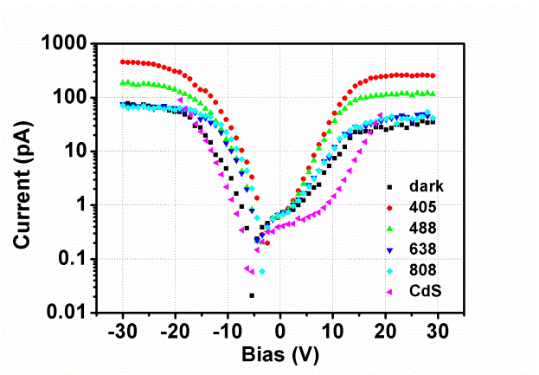
\includegraphics[width=0.6\textwidth]{figures/figure3_4}
%\caption[Photocurrent in Log scale.]{Photocurrent through junction in Log scale.
%\label{fig:fig3_4}}
%\end{figure}

Then, a detailed structural study of the junction was conducted using HRTEM imaging and electron diffraction analysis. The HRTEM images of a given CdS/p-Si axial heterojunction are depicted in Figure \ref{fig:fig3_2}. These confirm that both structures are perfect single crystals. The contact interface between two nanowires is atomically smooth. A thin transient graphitic layer is noticed between the wires. It has the origin similar to that mentioned above. In Figure \ref{fig:fig3_2}a, the left-hand-side panel shows the CdS nanowire, whereas the right-hand-side depicts the B-doped Si nanowire. Figures \ref{fig:fig3_2}b and \ref{fig:fig3_2}c present the entire crystallography of the CdS branch. Figure \ref{fig:fig3_2}d and \ref{fig:fig3_2}e present the crystal lattice of the constituting Si nanowire. Figure \ref{fig:fig3_2}f is the fast Fourier transform pattern of Figure \ref{fig:fig3_2}a. Figure \ref{fig:fig3_2}g is the selected area diffraction pattern taken at the junction interfacial portion. After the detailed structural analysis, which confirmed that high-quality axial heterojunction, constructed of two defect-free pure nanowire single crystals, had indeed been prepared, electrical and optoelectronic tests on it were promptly started. 

\begin{figure}  
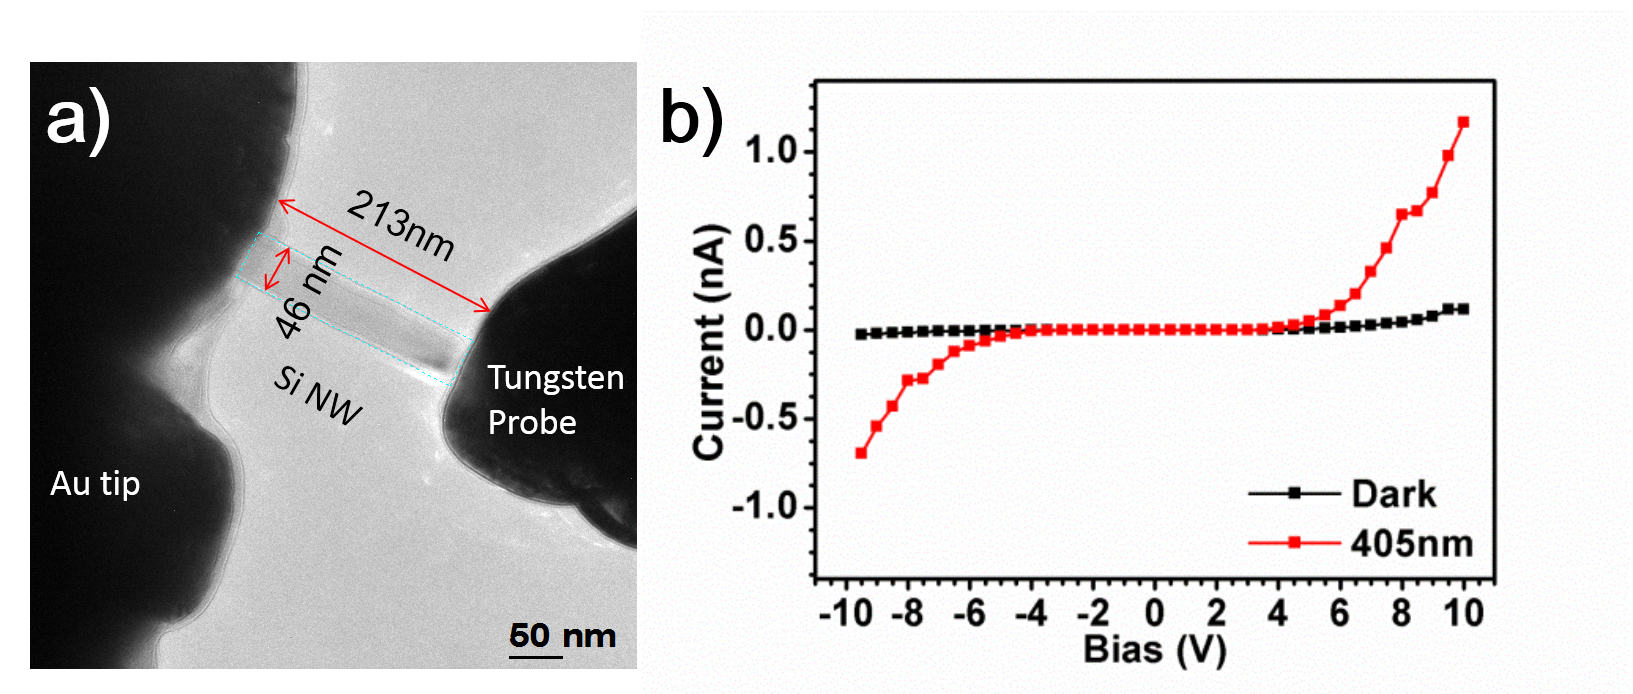
\includegraphics[width=\textwidth]{figures/figure3_s2}
\caption[TEM and currents of a Si NW]{(a) In situ alignment of a single B-doped Si nanowire for photocurrent measurements. (b) Dark current and photocurrent from the nanowire. 
\label{fig:fig3_s2}}
\end{figure}

While applying a voltage and illuminating the preformed CdS/p-Si heterojunction with a light through the optical fiber threaded inside the holder, dark current and photocurrent data were collected. Figure \ref{fig:fig3_3} illustrate a typical current – voltage diagram of a junction illuminated with lasers of 4 different wavelengths. The powers of all laser diodes were fixed to be the same, 13 mW. A photocurrent from the junction at 405 nm was larger than that at 488 nm, and much higher than those at 638 nm, and 808 nm, and the dark current. Because laser diode wavelengths of 405 nm, 488 nm, 638 nm and 808 nm correspond to energies of 3.06 eV, 2.54 eV, 1.94 eV and 1.53 eV, respectively, while CdS and Si nanowire band gaps are ~2.4 eV and ~1.5 eV, respectively, \cite{Fabbri2014}, the heterostructure light absorption at 3.06 eV and 2.54 eV must be more prominent than that at the energy <2.4 eV. The better photoresponse at 3.06 eV compared to that at 2.54 eV could reflect a complicated band diagram of the heterojunction which creates more light absorption capabilities at a higher energy, and thus results in numerous photo-induced carriers. 


The I-V curves of the CdS/p-Si axial junction, where CdS is assumed to be an n-type semiconductor (due to S vacancies), and B-doped Si as a p-type semiconductor, did not display ideal p-n junction parameters. In the forward bias regime, below 10 V, the I-V curves reveal low currents, and the currents tend to be saturated at a bias higher than 20 V. In the reverse bias regime, the currents also display a saturation tendency, over 30 V. 

\begin{figure}  
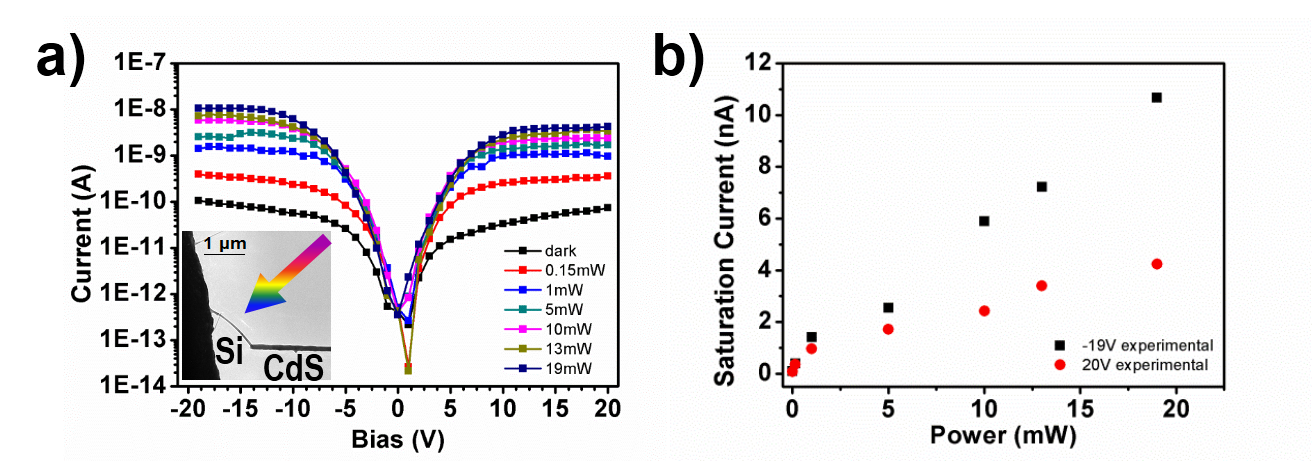
\includegraphics[width=\textwidth]{figures/figure3_5}
\caption[Photocurrent at different power]{Saturation trends of photocurrent and dark current at different of light intensities. (a) I–V curves recorded at various powers of lasers; the inset illustrates the low-magnification TEM image of the structure under testing; the multi-coloured arrow directs the light incidence; (b) current-laser power plots at the two selected biases.
\label{fig:fig3_5}}
\end{figure}

For a comparison it should be noted that, for an individual  CdS nanowire or a B-doped Si nanowire, saturation did not occur up to 10 V, as marked in Figure \ref{fig:fig3_3} and Figure \ref{fig:fig3_s2}. Once a bias larger than 10 V had been applied to a single CdS or Si nanowire, their structural breakdown readily happened. This was due to resistive heating at a high current density. \cite{Wu2004} In my experiments, the single crystalline nanowires (having narrow contact areas with the electrodes) were particularly vulnerable to current densities larger than ~104 $A\cdot cm^{-2}$. Therefore, it is apparent that the CdS/p-Si junction effectively hampered the current density at a high bias, and thus the whole junction ensemble is not deteriorated. 


Test experimental runs were performed to understand the associated factors responsible for the current saturation. As marked in Figure \ref{fig:fig3_5}, by recording  photocurrents for different light intensities at 488 nm, we observed that photocurrents and dark current of the CdS/p-Si axial nanowire junction at changing laser powers were saturated accordingly.The saturated currents were proportional to the laser diode power. Such phenomenon implies that the CdS/p-Si junction transfers light intensity into an electrical signal with the unmatched voltage tolerance. As shown in Figure \ref{fig:fig3_s3}, another junction with a smaller contact area, which was irradiated by a 405 nm laser at 13 mW, also demonstrated a profound saturation effect. The photocurrent saturated at 5 V, the saturation current values were 15 nA and –75 nA. Therefore, it is likely that the junction contact conditions mainly determine the saturation threshold and the current value. Primarily, the photocurrents in nanowire photodetectors are proportional to the voltage \cite{577926470}, while, simultaneously, they are proportional to the light intensity. This implies that the voltage should be certain and stable within a decent tolerance for reliable light detection. Therefore, the currently built CdS/p-Si axial nanowire junctions reveal a good promise toward light intensity sensing not only because they can limit the current density at a high voltage, but also because they do not require an entirely stable voltage. 

\begin{figure}  
\centering
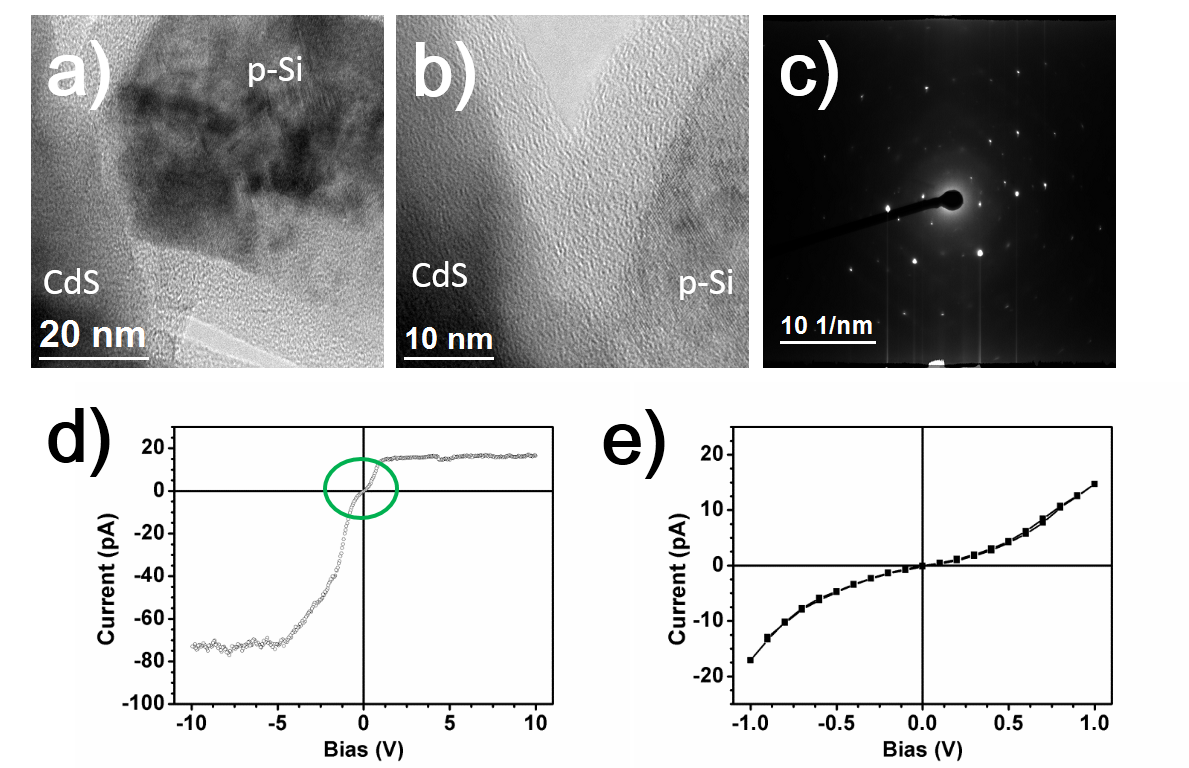
\includegraphics[width=0.9\textwidth]{figures/figure3_s3}
\caption[Another junction]{ (a,b) TEM images, and (c) SAED pattern of a CdS/p-Si junction having the narrow contact region. (d-e) Photocurrent measurements on this junction. 
\label{fig:fig3_s3}}
\end{figure}

The observed phenomenon of photocurrent saturation at the high bias levels seems to to be analogous to that discovered for a planar Metal-Semiconductor-Metal (MSM) photodetector \cite{577926472}, electron beam excited CdS single crystals \cite{Dervos2004}, a model p-n junction \cite{577926474} and a p-n junction solar cell \cite{Gu2005}. Firstly, the electron beam excitation mechanism should be not taken into account, because the electron beam was shut during the measurements, and it did not have a continuous effect on the material photocurrent \cite{Dervos2004}. Secondly, the prepared CdS nanowires were confirmed to be defect-free single crystals with a marginal number of sulfur vacancies, and, thus, they did not operate as a heavily doped donor. For an ideal p-n junction, the dark current is written as: 
$$I=I_s\left(e^\frac{V_D}{nV_t}-1\right)\eqno{(1)}$$

Equation ($1$) is named as Shockley’s diode equation \cite{577926477} and the dark current density of a non-ideal diode could be expressed as: 
$$J_F\approx-\frac{q(2D_p)N_i}{L_p}e^\frac{qV}{mk_0T}\eqno{(2)}$$
The factor $m$ in Equation ($2$) is changeable. Under circumstances of very low and very large biases, $m = 2$, and $J_F\propto e^\frac{qV}{k0T}$, the recombination current or the high injection takes an effect, current densities increase linearly; when bias is on a medium level, $m=1$, $J_F\propto e^\frac{qv}{2k0T}$, the diffusion current becomes important, and the current density exponentially increases. This is similar to the observed I-V curve trends, but Equation (2) does neither exactly explain the photocurrent saturation phenomenon nor the relationship between the saturation current value and incident light intensity. From the theory of photocurrent saturation developed by Mohammad and Abidi \cite{577926474}, for lightly degenerated semiconductors, where spatial variations of effective mass, carrier lifetime their mobility and diffusivity, and dielectric constant, are marginal and may be neglected, the total current is expressed as: 
$$I=Aqg\left ( L_{n}^{*}+L_{p}^{*} \right )-\frac{\left ( e^{\frac{qV_j}{kT}-1} \right )\cdot \left (  I_0+I_{0}^{'} e^{-z} \right )}{1-e^{-2z+z_1+z2}}\eqno{(3)}$$
where, 
$$I_0=\frac{qA}{\tau_a}(n_0(x_{p2})L_n^*+p_0(x_{n2})L_p^*)$$
$$I_0=\frac{qA}{\tau_a}(n_0(x_{p2})L_p^*e^{z2}+p_0(x_{n2})L_n^*e^{z1})$$
$$L_n^*=L_p^*=L_a=\sqrt{D_a\tau_a}$$
$D_a$, $\tau _{a}$ and $g$ are defined as ambipolar-diffusion coefficient, ambipolar lifetime and amibipolar-carrier generation rate, respectively\cite{577926474}. We do not neglect injection, $V_j, V_d$, and  it is considered that $z_1=z_2=0$, $z=\frac{q}{kT}(V_d-V_j)$ in nondegenerated semiconductors with uniform doping, Equation (3) could be written as: 
$$I=2qAg\sqrt{D_a\tau_a}-k_v(n_0x_{p2}+p_0x_{n2})\eqno{(4)}$$
$k_v$ is defined as a factor to simplify the equation. The first term in the right-hand side of this formula represents the uncompensated current relative to light intensity, and the second term stands for the reduction of this photocurrent owing to spatial dependence of band structure of the junction and the junction potential produced by strong injection. For a single B-doped Si or a defect-free CdS nanowire, the current density increases with bias, as this does for a standard semiconductor nanowire with Schottky contacts. However, for the CdS/p-Si nanowire junctions with a limited junction area and under a large bias, the second term in Equation (4) becomes negligible, and, thus, the photocurrent does not increase with a bias but does with the light intensity. 
The observed saturation current values in accord with the incident light intensities can be explained based on several factors. Because a sufficient bias must be applied to have the flat band at the anode and separate the generated carriers, after the threshold bias, the photocurrent started to notably rise, but when the bias is large enough, effective carriers produced by the incident light become saturated for transmission. In addition, we claim that the CdS/p-Si axial nanowire heterostructures are particularly sensitive to 3 factors: the relative dimensions of the two building blocks (this affects carrier mobility), carrier density and light absorption efficiency; interface crystallography (which also determines the mobility), junction parameters; and light intensity; that influences the photocurrent saturation value. 

%table with figure number
\begin{table}[ht]
\centering
\begin{tabular}{|c|c|c|c|c|c|}
\hline
Experiment No. & 1 & 2 & 3 & 4 & 5\\
\hline
CdS NW Length ($\mu$m) & 3 & 0.8 & 1.6 & 10 & 13\\
CdS NW Diameter (nm) & 240 & 38 & 135 & 187 & 120\\
Si NW Length ($\mu$m) & 0.9 & 1.5 & 1.3 & 0.2 & 1\\
Si NW Diameter (nm) & 55 & 44 & 44 & 46 & 63\\
Photoresponse detected & 26/26 & 22/22 & 16/16 & 57/57 & 16/16\\
Saturation current positive (nA) & 16 & 0.50 & 3.2 & 0.12 & 0.16\\
Saturation current negative (nA) & -27 & -0.69 & -7.2 & -0.19 & -0.2\\
\hline
\end{tabular}
\caption[Reproducibility of the saturation effect]{Five independent CdS/p-Si nanowire axial heterojunctions exhibiting the saturation effect all having varying values of sizes and currents. 
\label{table:3_1}}
\end{table}

Over this work I fabricated and thoroughly tested 5 distinct CdS/p-Si nanowire junctions. All of them exhibited the regarded saturation effects with notably varying parameters, as depicted in Table \ref{table:3_1}. The results imply that the saturation effects are natural and highly reproducible during \emph{in situ} TEM. 

\section{Conclusions}
To sum up, an original {\em in situ} HRTEM technique to construct individual axial nanowire junctions (perfectly emphasizing the modern {\em nanoarchitectonics} concept) has been developed for the first time. 
{\em In situ} HRTEM and in-parallel structural characterizations and optoelectronic tests highlight the photosensing properties of the single-crystalline axial CdS/p-Si nanowire junctions. They exhibit good selectivity toward the light frequencies higher than those of the yellow range. The junctions possess a specific photocurrent saturation effect; this can be employed in low-consumption light intensity sensing and integrated tunable voltage-driven applications owing to the effects of current limitations and excellent tolerance toward possibly unreliable and unstable bias. \\
The developed nanoarchitectonics-based approach employing \textit{in situ} structural design and measurements gives a strong motivation for setting new operational principles of single crystalline nano-devices. 
Moreover, it is also envisaged that the near-field scanning technique can be also integrated for the constructed system for even better uncovering the exciting nanoscale optoelectronic phenomena.\cite{Gu2005,Xiang2012}.



